\pagebreak
\section{Cursograma de Ventas}
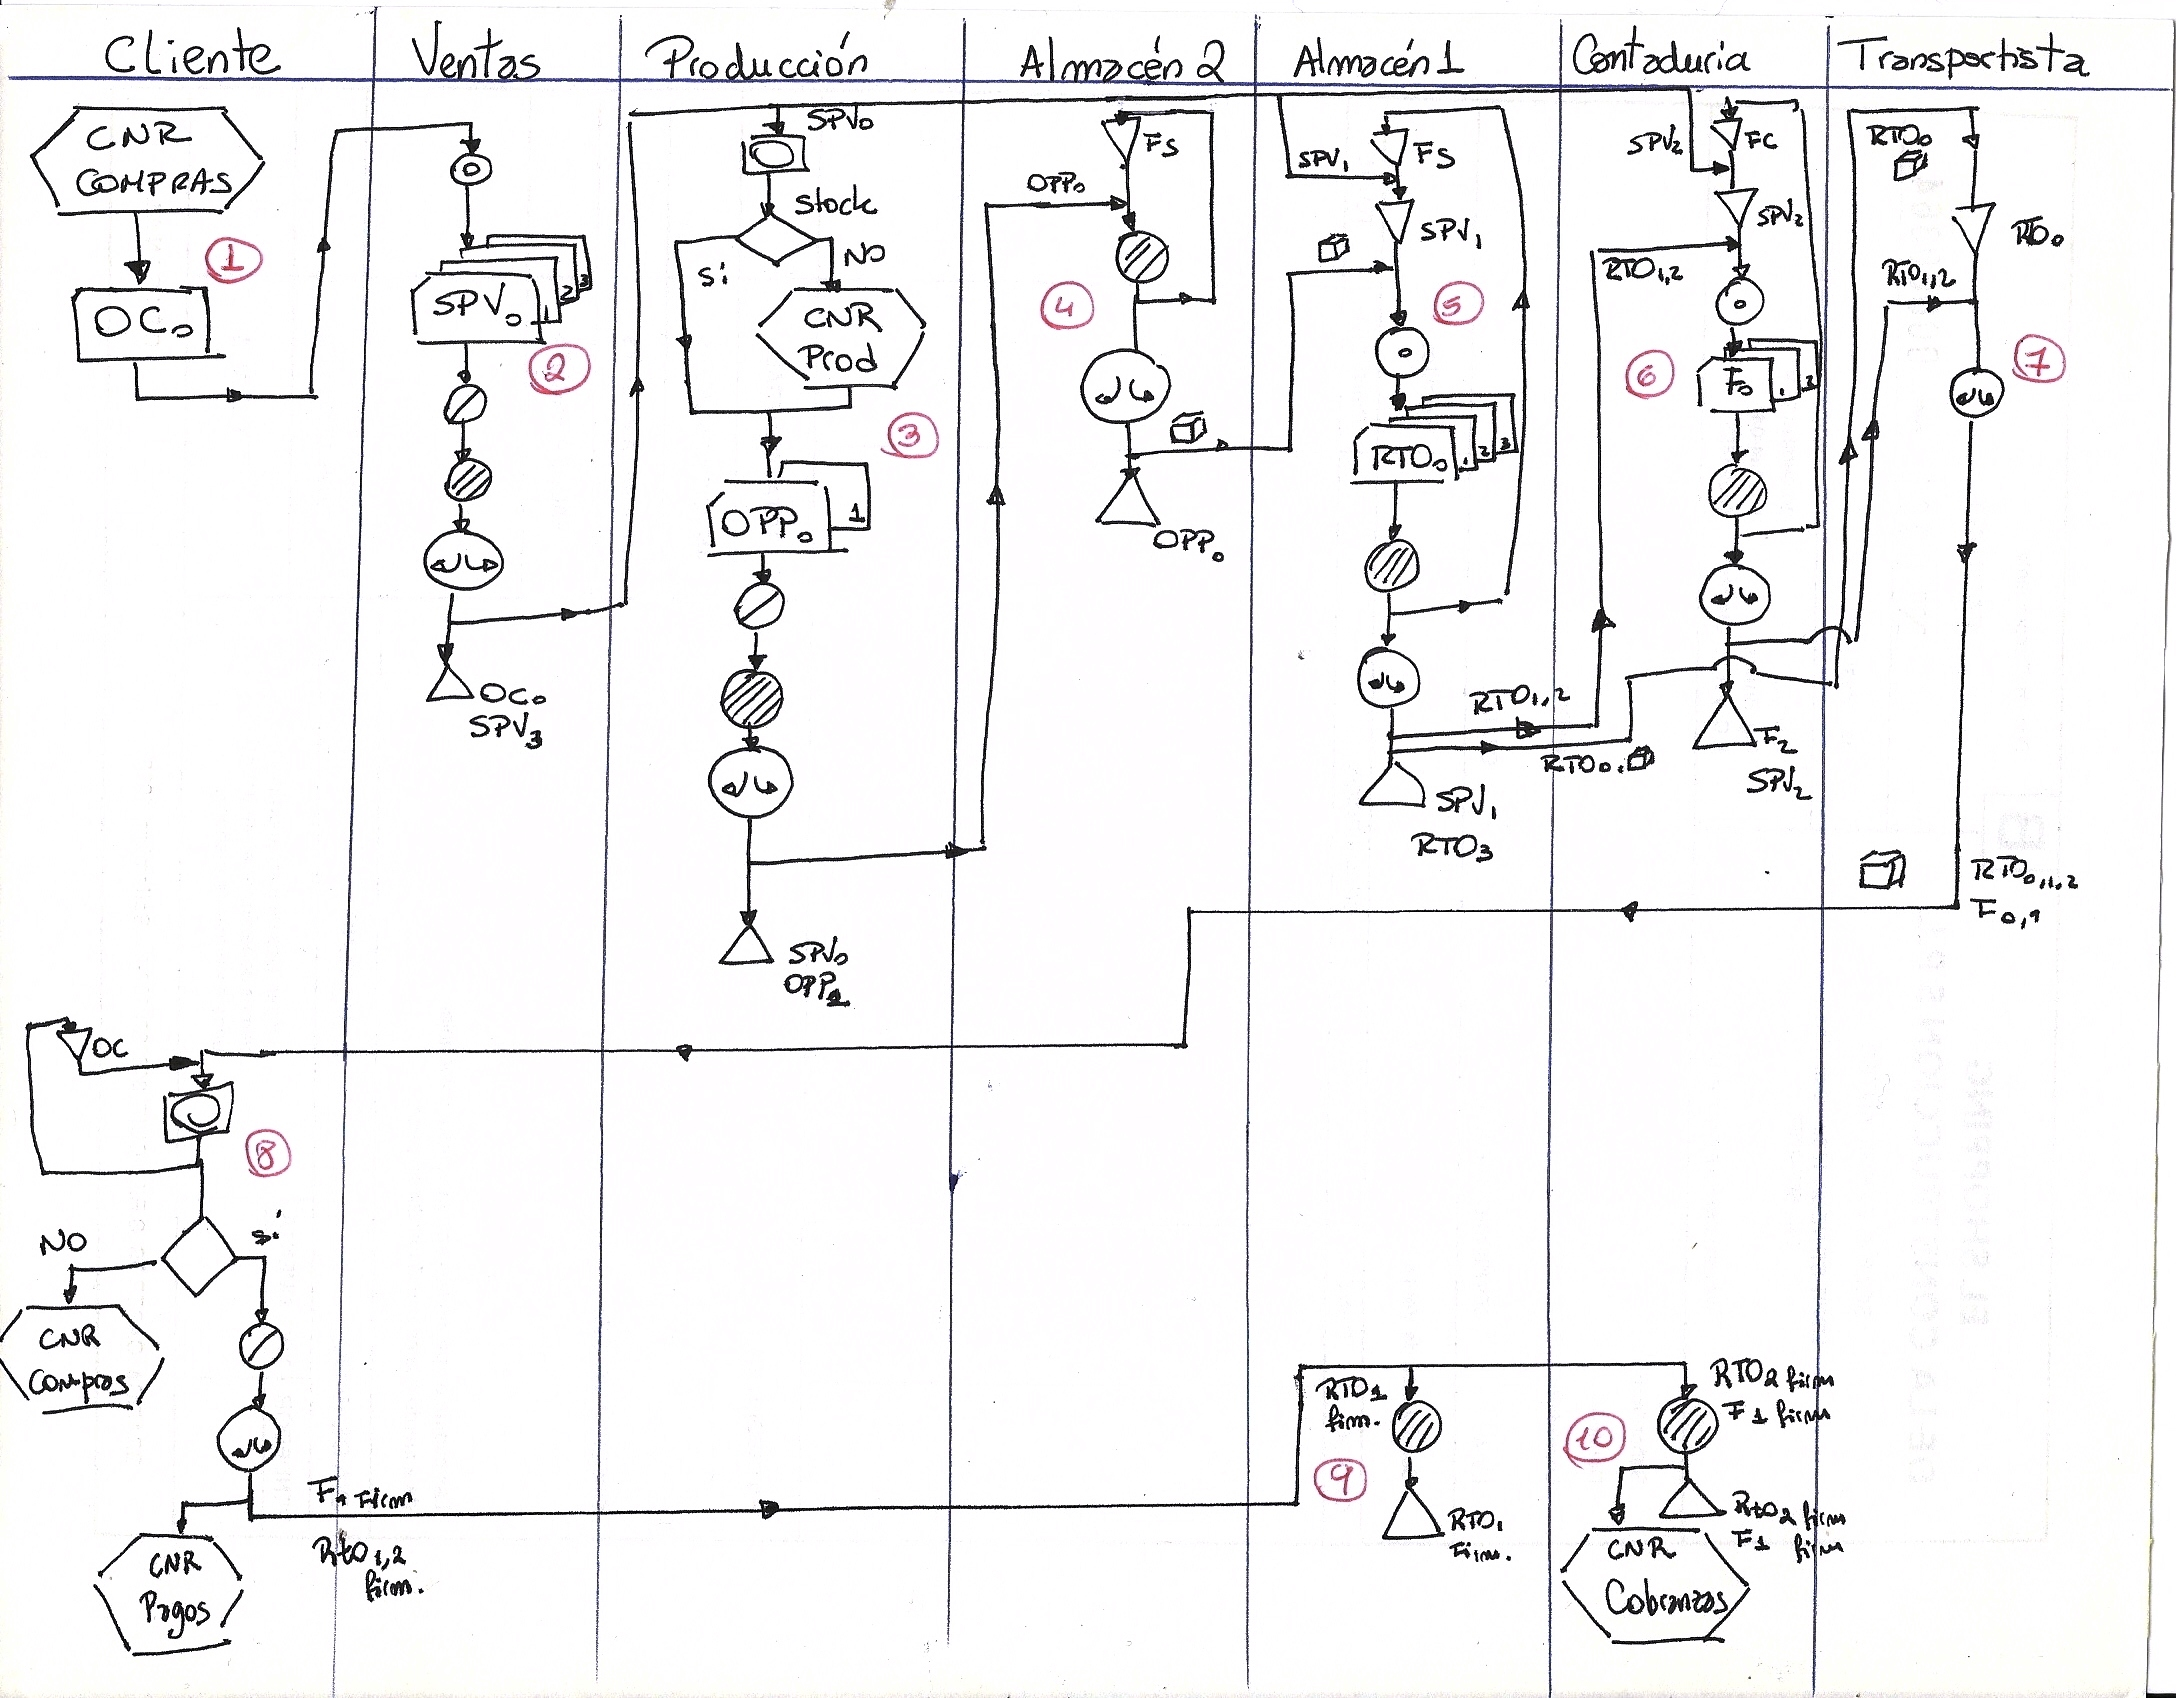
\includegraphics[scale=0.65, angle=90]{Empresa/Circuitos/Ventas/ventas.jpg}

\pagebreak
\section{Procedimiento de Ventas}
 \begin{description}
	\item[Cliente] El cliente solicita un pedido emitiendo una 'Orden de Compra' (OC).
	\item[Ventas] El área de ventas recibe la 'Orden de Compra' de parte del cliente y de esta manera genera la 'Solicitud de Pedido de Ventas' (SPV) especificando los detalles de la venta como por ejemplo, productos y plazo de entrega tentativo. Firma la SPV y envía una copia a Producción. Registra en el sistema del acciones realizas y archiva en forma definitiva la 'Orden de Compra'.
	\item[Producción] Producción recibe la SPV y verifica que cuenta con stock suficiente. De no poseer stock necesario se procede a realizar el 'Circuito no relevado de de Producción' (CNR Producción). En caso de contar con el producto solicitado, genera una 'Orden de Pedido de Productos' y la envía a Almacén 2 (Almacén de roductos terminados).  Registra en el sistema del acciones realizas y archiva en forma definitiva la 'Solicitud de Pedido de Ventas'. 
	\item[Almacén 2] Almacén 2 recibe la 'Orden de Pedido de Productos', ya cuenta con el producto (ya sea porque tenía stock o porque lo ha producido especialmente) y envía el producto junto con la documentación a Almacén 1. Registra en el sistema del acciones realizas.
	\item[Almacén 1] Almacén 1 prepara los productos para su entrega y genera el 'Remito' correspondiente por triplicado. Entrega el producto al Transportista con los remitos original y copia para que sean firmados por el cliente, y entrega la otra copia a Contaduría. Registra en el sistema del acciones realizas y archiva en forma definitiva la 'Orden de Pedido de Productos'.
	\item[Contaduría] Contaduría genera un listado de remitos sin facturar asociados a la venta, y genera la 'Factura' correspondiente por duplicado. Registra en el sistema del acciones realizas y envía el original y copia de la factura al Transportista para su envío.
	\item[Transportista] Transportista recibe los remitos, las facturas y la carga a ser enviada. Envía el pedido junto con la documentación al cliente. 
	\item[Cliente] El cliente recibe los remito, las facturas y el pedido. Chequea la mercadería recibida junto con los documentos original, y firmas las copias de los mismos.
	\item[Almacén 1] Almacen 1 recibe la copia del remito firmado por el cliente y cierra la orden de pedido. 
	\item[Contaduría] Contaduría recibe la copia de la factura y el remito firmado por el cliente y la asienta como recibida por el cliente. El pago de la factura es parte del 'Circuito no relevado de Cobranzas' (CNR Cobranzas)
\end{description}

\subsection{Entrevista}
Luego de analizar los diagramas de procedimiento de alto nivel del proceso de ventas que la empresa puso a nuestra disposici\'on, surgi\'o la necesidad de realizar una entrevista para aclarar ciertos puntos que no quedaban claros con nuestro contacto. Los puntos en cuesti\'on fueron los siguientes:
\begin{description}
 \item \underline{Ventas a Clientes}: \\
	Es el Centro de Atenci\'ion al Cliente (\textit{CAC}) quien interact\'ua con los clientes para realizar las ventas. Las ventas a clientes las ventas se realizan a partir de un pedido de cotizaci\'on confeccionado por el CAC. Posteriormente, el CAC formaliza el pedido de venta al recibir una Orden de Compra del cliente. Internamente, el CAC realiza una Solicitud de Pedido de Ventas (SPV).  \\
	Para el caso de los Distribuidores, ellos reciben la lista de precios y pueden formalizar directamente la Orden de Compra, es decir, que no hay cotizaci\'on previa del CAC.
 \item \underline{Registro de Clientes}: \\
	La empresa mantiene un registro de los clientes, y las transacciones que realizan con la empresa, mediante el sistema ERP Bejerman. Esta base de datos es actualizada por el \'area de Ventas, a trav\'es del \textit{CAC} y es consultada por todas las personas de la empresa que tienen habilitada esa funci\'on dentro de los m\'odulos del sistema inform\'atico. 
 \item \underline{Moviemiento de Materiales}: \\
	El medio de comunicaci\'on entre almacenes es electr\'onico, es decir, se realiza a trav\'es del sistema Bejerman, y as\'i se realizan las transferencias ``inter-dep\'osito''. Los documentos internos s\'olo se imprimen en papel cuando resulta necesario, y en casos particulares. En una \'epoca se utilizaban fichas y vale de materiales, pero fueron reemplazados por el sistema inform\'atico. Lo mismo sucede con el sector de Producci\'on, que maneja el movimiento de materiales mediante el sistema Bejerman.\\
	El sector de Producci\'on recibe por sistema la carga de datos del \'area de Ventas (CAC), formaliz\'andolo como ``Orden de Pedido''. En funci\'on a ello elabora una ``Orden de Montaje'', donde el sistema carga los elementos necesarios para confeccionar el pedido solicitado (las distintas partes y piezas para armar la luminaria). Terminado el producto, \'este se declara en el Dep\'osito Producto Terminado (02). Luego, el sector de Almacenes realiza por sistema la transferencia del producto, desde el 02 al Deposito Principal (01), y es desde aqu\'i que el \'area de Expedici\'on puede generar posteriormente el remito para despachar la mercader\'ia.  
	El transportista carga la mercader\'ia seg\'un la información emanada de los remitos, controlando f\'isicamente la carga.  Luego se le confecciona una Hoja de Ruta con el itinerario diario y por ultimo se le emite un permiso ante el ARBA, en caso que la mercader\'ia que se transporte supere los \$20.000.-   
\end{description}

\pagebreak
\section{Manual del Cursograma de Ventas}

\begin{center}\textbf{Sectores intervinientes}\end{center}
\begin{itemize}
  \item Cliente
  \item Ventas
  \item Producción
  \item Almacen 2
  \item Almacen 1
  \item Contaduría
  \item Transportista
\end{itemize}

\begin{center}
  \textbf{Documentos}
  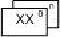
\includegraphics{./Images/Simbolos/simbolo-Documentos.png}
\end{center}
\begin{enumerate}
  \item Orden de Compra (OC).
  \item Solicitud de Pedido de Ventas (SPV).
  \item Orden de Pedido de Productos (OPP).
  \item Remito (RTO).
  \item Factura (F).
\end{enumerate}

\begin{center}
  \textbf{Emisión de Documentos}
  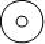
\includegraphics{./Images/Simbolos/simbolo-Emision-de-Documentos.png}
\end{center}
\begin{enumerate}
  \item Cliente emite una Orden de Compra.
  \item Ventas emite una Solicitud de Pedido de Ventas. 
  \item Producción emite una Orden de Pedido de Productos.
  \item Almacén 1 emite remitos por triplicado.
  \item Contaduría emite facturas por duplicado.
\end{enumerate}

\begin{center}
  \textbf{Firma}
  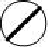
\includegraphics{./Images/Simbolos/simbolo-Firma.png}
\end{center}
\begin{enumerate}
  \item Ventas firma la Solicitud de Pedido de Ventas.
  \item Producción firma la Orden de Pedido de Productos.
  \item Almacén 2 firma la Orden de Pedido de Productos.
  \item Cliente firma las copias de remito y factura.
\end{enumerate}

\begin{center}
  \textbf{Distribución}
  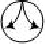
\includegraphics{./Images/Simbolos/simbolo-Distribucion.png}
\end{center}
\begin{enumerate}
  \item Ventas distribuye Solicitud de Pedido de Ventas.
  \item Producción distribuye Orden de Pedido de Productos.
  \item Almacen 2 distribuye Orden de Pedido de Productos junto con el pedido.
  \item Almacen 1 remitos por triplicado junto con el pedidoo.
  \item Contaduría distribuye las copias de los remitos y las facturas.
  \item Transportista distribuye los remitos, las facturas y el pedido.
  \item El Cliente distribuye las copias de remito y facturas firmadas.
\end{enumerate}

\begin{center}
  \textbf{Almacenamiento Transitorio}
  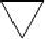
\includegraphics{./Images/Simbolos/simbolo-Almacenamiento-Transitorio.png}
\end{center}
\begin{enumerate}
  \item Cliente almacena Orden de Compra.
  \item Contaduría almacena una ficha del cliente.
  \item Transportista almacena los remitos, las facturas y el pedido.
\end{enumerate}

\begin{center}
  \textbf{Control y verificación}
  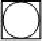
\includegraphics{./Images/Simbolos/simbolo-Control-y-Verificacion.png}
\end{center}
\begin{enumerate}
	\item Producción controla si cuenta con stock suficiente con la Solicitud de Pedido de Ventas.
	\item El cliente controla si el pedido recibio es realmente lo que pidió con la Orden de Compra.
\end{enumerate}
\pagebreak

\begin{center}
  \textbf{Decisión}
  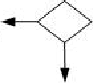
\includegraphics{./Images/Simbolos/simbolo-Decision.png}
\end{center}
\begin{enumerate}
  \item Producción controla el stock. De no poseer procede a realizar el 'Circuito no relevado de de Producción' (CNR Producción). En caso de contar con el producto solicitado, genera una 'Orden de Pedido de Productos'.
  \item Cliente controla el pedido recibido. En caso de existir algún inconveniente ejecuta parto de un 'Circuito no relevado de Compras'.
\end{enumerate}

\begin{center}
  \textbf{Registro}
  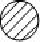
\includegraphics{./Images/Simbolos/simbolo-Registro.png}
\end{center}
\begin{enumerate}
  \item Ventas registra la venta en curso.
  \item Almacen 2 registra la entrega de mercadería.
  \item Almacen 1 registra la entrega de mercadería.
  \item Contaduría registra la emisión de la factura.
  \item Almacen 1 registra el arribo de la copia del remito firmada por el cliente.
  \item Contaduría registra el arribo de la copia de la factura firmada por el cliente.  
\end{enumerate}

\begin{center}
  \textbf{Almacenamiento definitivo}
  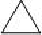
\includegraphics{./Images/Simbolos/simbolo-Almacenamiento-Definitivo.png}
\end{center}
\begin{enumerate}
  \item Ventas almacena la Orden de Compra.
  \item Producción almacena la Solicitud de Pedido de Ventas.
  \item Almacen 1 almacena la Orden de Pedido de Productos y la copia firmada del remito.
  \item Contaduría almacena la copia de la factura y el remito firmada.  
\end{enumerate}

\begin{center}
  \textbf{Circuito no relevado}
  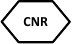
\includegraphics{./Images/Simbolos/simbolo-CNR.png}
  % simbolo-CNR.png: 73x44 pixel, 96dpi, 1.93x1.16 cm, bb=0 0 55 33
\end{center}
\begin{enumerate}
  \item Compras (circuito del cliente).
  \item Pagos (circuito del cliente).
  \item Cobranzas.
\end{enumerate}

\pagebreak
\section{Formularios de Ventas}

\subsection{Factura}
\begin{center}
 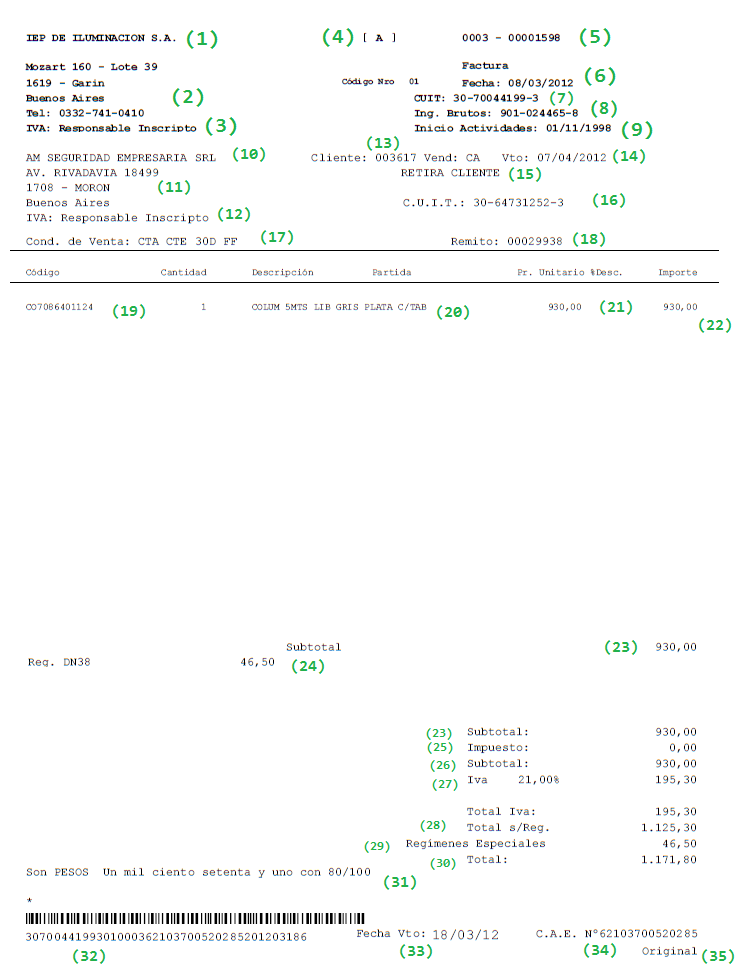
\includegraphics[scale=0.85,keepaspectratio=true]{./Images/FormulariosIEP/Factura.png}
 % Factura.png: 749x973 pixel, 96dpi, 19.82x25.75 cm, bb=0 0 562 730
\end{center}
\begin{itemize}
  \item \textbf{Objetivo:} Con este documento se notifica al cliente que efectu\'o la compra el monto total a pagar. Se especifica el remito asociado, los productos comprados con detalle de precios, los impuestos incluidos y las condiciones de pago.
  \item \textbf{Alcance:} Es un documento entre la empresa y el cliente.
  \item \textbf{Emisor:} Contadur\'ia.
  \item \textbf{Cantidad de Copias Emitidas:} Original y Copia.
  \item \textbf{Sector receptor:} Expedici\'on, para su env\'io al cliente.
\end{itemize}
\subsubsection{Descripci\'on campos de la Factura}
\begin{enumerate}
  \item Empresa emisora: Raz\'on Social de la empresa
  \item Empresa emisora: Información de Sucursal. Domicilio y N\'umero de Tel\'efono
  \item Empresa emisora: Responsabilidad frente al IVA
  \item Tipo de Factura (A en este caso)
  \item N\'umero de Factura
  \item Fecha de emisi\'on
  \item Empresa emisora: CUIT
  \item Empresa emisora: C\'odigo de Ingresos Brutos
  \item Empresa emisora: Fecha de inicio de actividades
  \item Cliente: Raz\'on Social 
  \item Cliente: Domicilio
  \item Cliente: Responsabilidad frente al IVA
  \item C\'odigo del cliente al que se le factura y C\'odigo de Vendedor (Opcional)
  \item Vencimiento de la Factura
  \item Condici\'on de entrega
  \item Cliente: CUIT
  \item Condici\'on de Venta / Tipo de Pago.
  \item Remito asociado a la Venta.
  \item Detalle de la factura: C\'odigo interno del \'item, Cantidad del \'item
  \item Detalle de la factura: Descripci\'on del \'item. La partida asociada es opcional
  \item Detalle de la factura: Precio unitario del \'item. El descuento del \'item es opcional.
  \item Detalle de la factura: Precio total del \'item (cantidad * precio unitario)
  \item Detalle de la factura: Subtotal de items (suma de los totales de \'item)
  \item Detalle de la factura: Detalle de Regímenes Especiales que aplican.
  \item Total de Impuestos que aplican a la venta (sin IVA).
  \item Subtotal con Impuestos y sin IVA.
  \item IVA discriminado.
  \item Subtotal con Impuestos e IVA, sin Reg\'imenes Especiales.
  \item Total de Reg\'imenes Especiales.
  \item Total del Importe de la Factura.
  \item Importe de la factura en palabras.(Opcional)
  \item C\'odigo de Barras de la factura. El c\'odigo tambi\'en se encuentra en forma num\'erica. 
  \item Fecha de vencimiento del C\'odigo de Impresi\'on
  \item CAE: C\'odigo de Autorizaci\'on Electr\'onico.
  \item Copia de la facura: Original, Copia, Triplicado, etc
\end{enumerate}

\subsection{Remito}
\begin{center}
 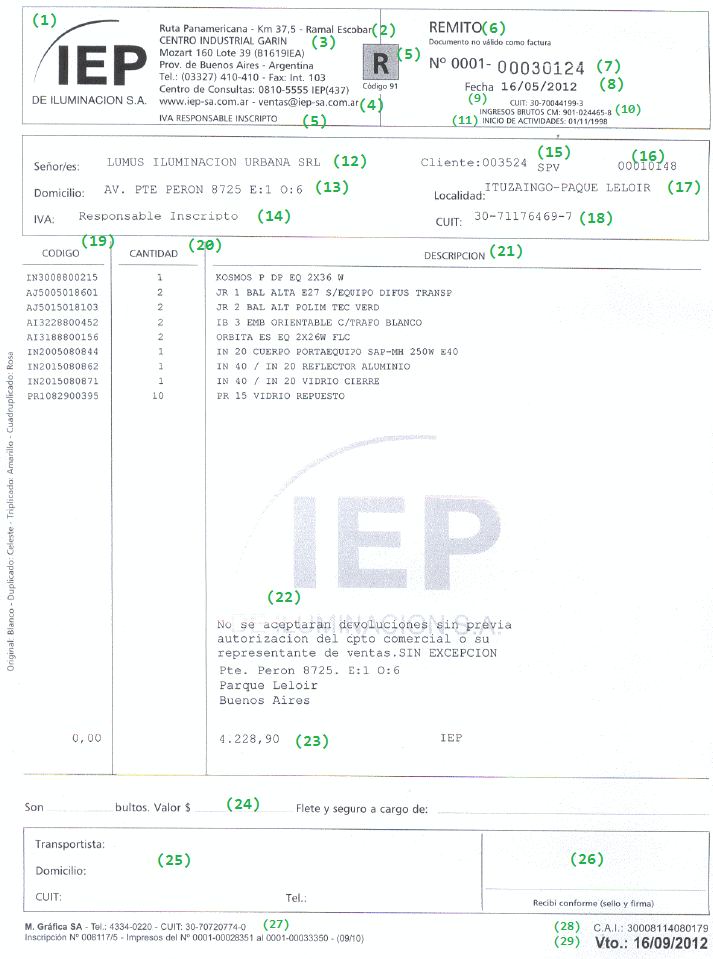
\includegraphics[scale=0.90,keepaspectratio=true]{./Images/FormulariosIEP/Remito.png}
 % Remito.png: 713x959 pixel, 96dpi, 18.87x25.38 cm, bb=0 0 535 720
\end{center}
\begin{itemize}
  \item \textbf{Objetivo:} En este documento se detallan los productos a ser enviados al cliente. No se incluyen detalles de precios y se especifica la contidad de bultos.
  \item \textbf{Alcance:} Es un documento entre la empresa y el cliente.
  \item \textbf{Emisor:} Almacén 1.
  \item \textbf{Cantidad de Copias Emitidas:} Original y Copia.
  \item \textbf{Sector receptor:} Expedición, para su envío al cliente.
 \end{itemize}
\subsubsection{Descripci\'on campos del Remito}

\pagebreak
\section{Normas de Control Interno de Ventas}
\begin{itemize}
 \item	{\bf Separaci\'on de funciones: } El encargado de ventas no debe poseer acceso a las registraciones de stock ni a la modificaci\'on de cuentas del cliente.
Quien vende no puede otorgar cr\'editos ni encargarse de la facturaci\'on. Dentro del sector de Ventas existe una clara divisi\'on entre la parte encargada de la atenci\'on a los clientes 
y la parte encargada de la venta en s\'i misma.
  \item	{\bf Aprobaci\'on de la venta: } Las pol\'iticas de ventas, otorgamiento de cr\'editos y precios son dispuestas por la Direcci\'on General.
La aprobaci\'on de la venta es realizada por el responsable de cr\'editos dado que es el que conoce el estado financiero de los clientes.
  \item	{\bf Movimiento de bienes: } La circulaci\'on de mercader\'ias est\'a respaldada por comprobantes firmados por el responsable del sector que los recibe. En los sectores de Producci\'on, 
Almac\'en 1 y 2 y Expedici\'on se documenta el transpaso de mercader\'ia utilizando el correspondiente m\'odulo del sistema inform\'atico de Bejerman.
  \item	{\bf Documentaci\'on prenumerada: } Toda documantaci\'on emitida debe estar prenumerada y se archivan en orden num\'erico, incluso las anuladas. Dado que todos los documentos se generan 
utilizando el sistema inform\'atico, resulta complicado alterar la numeraci\'on dado que la misma es autogenerada utilizando una secuencia.
  \item	{\bf Control de Facturaci\'on: } Contadur\'ia realiza un control cruzado de la facturaci\'on y remitos. Contadur\'ia siempre conserva una copia de las facturas y remitos emitidos. 
A su vez, realiza un control antes de que dichos documentos sean enviados al cliente.
\end{itemize}
